% Created by tikzDevice version 0.12 on 2019-04-27 02:35:12
% !TEX encoding = UTF-8 Unicode
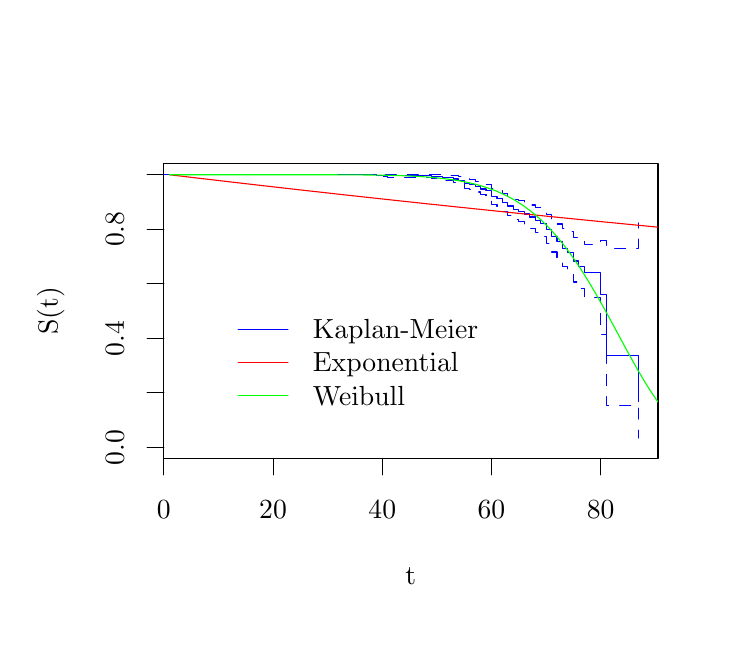
\begin{tikzpicture}[x=1pt,y=1pt]
\definecolor{fillColor}{RGB}{255,255,255}
\path[use as bounding box,fill=fillColor,fill opacity=0.00] (0,0) rectangle (252.94,216.81);
\begin{scope}
\path[clip] (  0.00,  0.00) rectangle (252.94,216.81);
\definecolor{drawColor}{RGB}{0,0,0}

\path[draw=drawColor,line width= 0.4pt,line join=round,line cap=round] ( 49.20, 61.20) -- (207.06, 61.20);

\path[draw=drawColor,line width= 0.4pt,line join=round,line cap=round] ( 49.20, 61.20) -- ( 49.20, 55.20);

\path[draw=drawColor,line width= 0.4pt,line join=round,line cap=round] ( 88.67, 61.20) -- ( 88.67, 55.20);

\path[draw=drawColor,line width= 0.4pt,line join=round,line cap=round] (128.13, 61.20) -- (128.13, 55.20);

\path[draw=drawColor,line width= 0.4pt,line join=round,line cap=round] (167.60, 61.20) -- (167.60, 55.20);

\path[draw=drawColor,line width= 0.4pt,line join=round,line cap=round] (207.06, 61.20) -- (207.06, 55.20);

\node[text=drawColor,anchor=base,inner sep=0pt, outer sep=0pt, scale=  1.00] at ( 49.20, 39.60) {0};

\node[text=drawColor,anchor=base,inner sep=0pt, outer sep=0pt, scale=  1.00] at ( 88.67, 39.60) {20};

\node[text=drawColor,anchor=base,inner sep=0pt, outer sep=0pt, scale=  1.00] at (128.13, 39.60) {40};

\node[text=drawColor,anchor=base,inner sep=0pt, outer sep=0pt, scale=  1.00] at (167.60, 39.60) {60};

\node[text=drawColor,anchor=base,inner sep=0pt, outer sep=0pt, scale=  1.00] at (207.06, 39.60) {80};

\path[draw=drawColor,line width= 0.4pt,line join=round,line cap=round] ( 49.20, 65.14) -- ( 49.20,163.67);

\path[draw=drawColor,line width= 0.4pt,line join=round,line cap=round] ( 49.20, 65.14) -- ( 43.20, 65.14);

\path[draw=drawColor,line width= 0.4pt,line join=round,line cap=round] ( 49.20, 84.85) -- ( 43.20, 84.85);

\path[draw=drawColor,line width= 0.4pt,line join=round,line cap=round] ( 49.20,104.55) -- ( 43.20,104.55);

\path[draw=drawColor,line width= 0.4pt,line join=round,line cap=round] ( 49.20,124.26) -- ( 43.20,124.26);

\path[draw=drawColor,line width= 0.4pt,line join=round,line cap=round] ( 49.20,143.96) -- ( 43.20,143.96);

\path[draw=drawColor,line width= 0.4pt,line join=round,line cap=round] ( 49.20,163.67) -- ( 43.20,163.67);

\node[text=drawColor,rotate= 90.00,anchor=base,inner sep=0pt, outer sep=0pt, scale=  1.00] at ( 34.80, 65.14) {0.0};

\node[text=drawColor,rotate= 90.00,anchor=base,inner sep=0pt, outer sep=0pt, scale=  1.00] at ( 34.80,104.55) {0.4};

\node[text=drawColor,rotate= 90.00,anchor=base,inner sep=0pt, outer sep=0pt, scale=  1.00] at ( 34.80,143.96) {0.8};

\path[draw=drawColor,line width= 0.4pt,line join=round,line cap=round] ( 49.20, 61.20) --
	(227.75, 61.20) --
	(227.75,167.61) --
	( 49.20,167.61) --
	( 49.20, 61.20);
\end{scope}
\begin{scope}
\path[clip] (  0.00,  0.00) rectangle (252.94,216.81);
\definecolor{drawColor}{RGB}{0,0,0}

\node[text=drawColor,anchor=base,inner sep=0pt, outer sep=0pt, scale=  1.00] at (138.47, 15.60) {t};

\node[text=drawColor,rotate= 90.00,anchor=base,inner sep=0pt, outer sep=0pt, scale=  1.00] at ( 10.80,114.41) {S(t)};
\end{scope}
\begin{scope}
\path[clip] ( 49.20, 61.20) rectangle (227.75,167.61);
\definecolor{drawColor}{RGB}{0,0,255}

\path[draw=drawColor,line width= 0.4pt,line join=round,line cap=round] ( 49.20,163.67) --
	(126.16,163.67) --
	(126.16,163.46) --
	(130.11,163.46) --
	(130.11,163.25) --
	(145.89,163.25) --
	(145.89,163.03) --
	(149.84,163.03) --
	(149.84,162.59) --
	(153.79,162.59) --
	(153.79,162.12) --
	(155.76,162.12) --
	(155.76,161.65) --
	(157.73,161.65) --
	(157.73,160.43) --
	(159.71,160.43) --
	(159.71,160.17) --
	(161.68,160.17) --
	(161.68,159.37) --
	(163.65,159.37) --
	(163.65,158.53) --
	(165.63,158.53) --
	(165.63,157.94) --
	(167.60,157.94) --
	(167.60,155.73) --
	(169.57,155.73) --
	(169.57,155.06) --
	(171.55,155.06) --
	(171.55,153.60) --
	(173.52,153.60) --
	(173.52,152.38) --
	(175.49,152.38) --
	(175.49,151.02) --
	(177.47,151.02) --
	(177.47,150.51) --
	(179.44,150.51) --
	(179.44,149.47) --
	(181.41,149.47) --
	(181.41,148.39) --
	(183.39,148.39) --
	(183.39,147.22) --
	(185.36,147.22) --
	(185.36,145.93) --
	(187.33,145.93) --
	(187.33,143.80) --
	(189.30,143.80) --
	(189.30,141.29) --
	(191.28,141.29) --
	(191.28,139.41) --
	(193.25,139.41) --
	(193.25,137.05) --
	(195.22,137.05) --
	(195.22,135.72) --
	(197.20,135.72) --
	(197.20,132.51) --
	(199.17,132.51) --
	(199.17,130.64) --
	(201.14,130.64) --
	(201.14,128.21) --
	(207.06,128.21) --
	(207.06,120.33) --
	(209.04,120.33) --
	(209.04, 98.25) --
	(220.88, 98.25) --
	(220.88, 81.70);

\path[draw=drawColor,line width= 0.4pt,dash pattern=on 4pt off 4pt ,line join=round,line cap=round] ( 49.20,163.67) --
	(126.16,163.67) --
	(126.16,163.04) --
	(130.11,163.04) --
	(130.11,162.66) --
	(145.89,162.66) --
	(145.89,162.31) --
	(149.84,162.31) --
	(149.84,161.64) --
	(153.79,161.64) --
	(153.79,160.99) --
	(155.76,160.99) --
	(155.76,160.35) --
	(157.73,160.35) --
	(157.73,158.77) --
	(159.71,158.77) --
	(159.71,158.45) --
	(161.68,158.45) --
	(161.68,157.44) --
	(163.65,157.44) --
	(163.65,156.40) --
	(165.63,156.40) --
	(165.63,155.68) --
	(167.60,155.68) --
	(167.60,153.02) --
	(169.57,153.02) --
	(169.57,152.21) --
	(171.55,152.21) --
	(171.55,150.47) --
	(173.52,150.47) --
	(173.52,149.03) --
	(175.49,149.03) --
	(175.49,147.40) --
	(177.47,147.40) --
	(177.47,146.79) --
	(179.44,146.79) --
	(179.44,145.54) --
	(181.41,145.54) --
	(181.41,144.26) --
	(183.39,144.26) --
	(183.39,142.86) --
	(185.36,142.86) --
	(185.36,141.31) --
	(187.33,141.31) --
	(187.33,138.76) --
	(189.30,138.76) --
	(189.30,135.74) --
	(191.28,135.74) --
	(191.28,133.48) --
	(193.25,133.48) --
	(193.25,130.57) --
	(195.22,130.57) --
	(195.22,128.92) --
	(197.20,128.92) --
	(197.20,124.89) --
	(199.17,124.89) --
	(199.17,122.53) --
	(201.14,122.53) --
	(201.14,119.35) --
	(207.06,119.35) --
	(207.06,105.92) --
	(209.04,105.92) --
	(209.04, 80.37) --
	(220.88, 80.37) --
	(220.88, 68.52);

\path[draw=drawColor,line width= 0.4pt,dash pattern=on 4pt off 4pt ,line join=round,line cap=round] ( 49.20,163.67) --
	(149.84,163.67) --
	(149.84,163.53) --
	(153.79,163.53) --
	(153.79,163.27) --
	(155.76,163.27) --
	(155.76,162.97) --
	(157.73,162.97) --
	(157.73,162.12) --
	(159.71,162.12) --
	(159.71,161.93) --
	(161.68,161.93) --
	(161.68,161.34) --
	(163.65,161.34) --
	(163.65,160.71) --
	(165.63,160.71) --
	(165.63,160.26) --
	(167.60,160.26) --
	(167.60,158.53) --
	(169.57,158.53) --
	(169.57,158.00) --
	(171.55,158.00) --
	(171.55,156.83) --
	(173.52,156.83) --
	(173.52,155.87) --
	(175.49,155.87) --
	(175.49,154.79) --
	(177.47,154.79) --
	(177.47,154.41) --
	(179.44,154.41) --
	(179.44,153.59) --
	(181.41,153.59) --
	(181.41,152.74) --
	(183.39,152.74) --
	(183.39,151.83) --
	(185.36,151.83) --
	(185.36,150.83) --
	(187.33,150.83) --
	(187.33,149.18) --
	(189.30,149.18) --
	(189.30,147.27) --
	(191.28,147.27) --
	(191.28,145.85) --
	(193.25,145.85) --
	(193.25,144.18) --
	(195.22,144.18) --
	(195.22,143.25) --
	(197.20,143.25) --
	(197.20,141.11) --
	(199.17,141.11) --
	(199.17,139.90) --
	(201.14,139.90) --
	(201.14,138.53) --
	(207.06,138.53) --
	(207.06,139.83) --
	(209.04,139.83) --
	(209.04,137.16) --
	(220.88,137.16) --
	(220.88,146.24);
\definecolor{drawColor}{RGB}{255,0,0}

\path[draw=drawColor,line width= 0.4pt,line join=round,line cap=round] ( 51.17,163.67) --
	( 53.15,163.43) --
	( 55.12,163.20) --
	( 57.09,162.97) --
	( 59.07,162.73) --
	( 61.04,162.50) --
	( 63.01,162.27) --
	( 64.99,162.04) --
	( 66.96,161.81) --
	( 68.93,161.58) --
	( 70.91,161.35) --
	( 72.88,161.12) --
	( 74.85,160.89) --
	( 76.83,160.66) --
	( 78.80,160.43) --
	( 80.77,160.20) --
	( 82.75,159.98) --
	( 84.72,159.75) --
	( 86.69,159.53) --
	( 88.67,159.30) --
	( 90.64,159.08) --
	( 92.61,158.85) --
	( 94.59,158.63) --
	( 96.56,158.41) --
	( 98.53,158.18) --
	(100.51,157.96) --
	(102.48,157.74) --
	(104.45,157.52) --
	(106.43,157.30) --
	(108.40,157.08) --
	(110.37,156.86) --
	(112.35,156.64) --
	(114.32,156.42) --
	(116.29,156.21) --
	(118.27,155.99) --
	(120.24,155.77) --
	(122.21,155.56) --
	(124.19,155.34) --
	(126.16,155.13) --
	(128.13,154.91) --
	(130.11,154.70) --
	(132.08,154.48) --
	(134.05,154.27) --
	(136.03,154.06) --
	(138.00,153.85) --
	(139.97,153.64) --
	(141.95,153.42) --
	(143.92,153.21) --
	(145.89,153.00) --
	(147.87,152.80) --
	(149.84,152.59) --
	(151.81,152.38) --
	(153.79,152.17) --
	(155.76,151.96) --
	(157.73,151.76) --
	(159.71,151.55) --
	(161.68,151.34) --
	(163.65,151.14) --
	(165.63,150.93) --
	(167.60,150.73) --
	(169.57,150.52) --
	(171.55,150.32) --
	(173.52,150.12) --
	(175.49,149.91) --
	(177.47,149.71) --
	(179.44,149.51) --
	(181.41,149.31) --
	(183.39,149.11) --
	(185.36,148.91) --
	(187.33,148.71) --
	(189.30,148.51) --
	(191.28,148.31) --
	(193.25,148.11) --
	(195.22,147.92) --
	(197.20,147.72) --
	(199.17,147.52) --
	(201.14,147.33) --
	(203.12,147.13) --
	(205.09,146.93) --
	(207.06,146.74) --
	(209.04,146.54) --
	(211.01,146.35) --
	(212.98,146.16) --
	(214.96,145.96) --
	(216.93,145.77) --
	(218.90,145.58) --
	(220.88,145.39) --
	(222.85,145.20) --
	(224.82,145.00) --
	(226.80,144.81) --
	(228.77,144.62);
\definecolor{drawColor}{RGB}{0,255,0}

\path[draw=drawColor,line width= 0.4pt,line join=round,line cap=round] ( 51.17,163.67) --
	( 53.15,163.67) --
	( 55.12,163.67) --
	( 57.09,163.67) --
	( 59.07,163.67) --
	( 61.04,163.67) --
	( 63.01,163.67) --
	( 64.99,163.67) --
	( 66.96,163.67) --
	( 68.93,163.67) --
	( 70.91,163.67) --
	( 72.88,163.67) --
	( 74.85,163.67) --
	( 76.83,163.67) --
	( 78.80,163.67) --
	( 80.77,163.67) --
	( 82.75,163.67) --
	( 84.72,163.67) --
	( 86.69,163.67) --
	( 88.67,163.67) --
	( 90.64,163.67) --
	( 92.61,163.67) --
	( 94.59,163.67) --
	( 96.56,163.67) --
	( 98.53,163.67) --
	(100.51,163.66) --
	(102.48,163.66) --
	(104.45,163.66) --
	(106.43,163.66) --
	(108.40,163.65) --
	(110.37,163.65) --
	(112.35,163.64) --
	(114.32,163.64) --
	(116.29,163.63) --
	(118.27,163.62) --
	(120.24,163.60) --
	(122.21,163.58) --
	(124.19,163.56) --
	(126.16,163.53) --
	(128.13,163.50) --
	(130.11,163.46) --
	(132.08,163.41) --
	(134.05,163.36) --
	(136.03,163.29) --
	(138.00,163.21) --
	(139.97,163.11) --
	(141.95,163.00) --
	(143.92,162.87) --
	(145.89,162.72) --
	(147.87,162.54) --
	(149.84,162.33) --
	(151.81,162.09) --
	(153.79,161.82) --
	(155.76,161.50) --
	(157.73,161.14) --
	(159.71,160.72) --
	(161.68,160.25) --
	(163.65,159.71) --
	(165.63,159.11) --
	(167.60,158.42) --
	(169.57,157.66) --
	(171.55,156.79) --
	(173.52,155.83) --
	(175.49,154.76) --
	(177.47,153.57) --
	(179.44,152.25) --
	(181.41,150.80) --
	(183.39,149.21) --
	(185.36,147.46) --
	(187.33,145.56) --
	(189.30,143.50) --
	(191.28,141.26) --
	(193.25,138.86) --
	(195.22,136.29) --
	(197.20,133.55) --
	(199.17,130.64) --
	(201.14,127.57) --
	(203.12,124.36) --
	(205.09,121.02) --
	(207.06,117.56) --
	(209.04,114.01) --
	(211.01,110.40) --
	(212.98,106.74) --
	(214.96,103.08) --
	(216.93, 99.44) --
	(218.90, 95.87) --
	(220.88, 92.40) --
	(222.85, 89.06) --
	(224.82, 85.89) --
	(226.80, 82.91) --
	(228.77, 80.17);

\path[] ( 67.05,119.84) rectangle (167.29, 71.84);
\definecolor{drawColor}{RGB}{0,0,255}

\path[draw=drawColor,line width= 0.4pt,line join=round,line cap=round] ( 76.05,107.84) -- ( 94.05,107.84);
\definecolor{drawColor}{RGB}{255,0,0}

\path[draw=drawColor,line width= 0.4pt,line join=round,line cap=round] ( 76.05, 95.84) -- ( 94.05, 95.84);
\definecolor{drawColor}{RGB}{0,255,0}

\path[draw=drawColor,line width= 0.4pt,line join=round,line cap=round] ( 76.05, 83.84) -- ( 94.05, 83.84);
\definecolor{drawColor}{RGB}{0,0,0}

\node[text=drawColor,anchor=base west,inner sep=0pt, outer sep=0pt, scale=  1.00] at (103.05,104.40) {Kaplan-Meier};

\node[text=drawColor,anchor=base west,inner sep=0pt, outer sep=0pt, scale=  1.00] at (103.05, 92.40) {Exponential};

\node[text=drawColor,anchor=base west,inner sep=0pt, outer sep=0pt, scale=  1.00] at (103.05, 80.40) {Weibull};
\end{scope}
\end{tikzpicture}
